\documentclass[12pt]{article}
%\usepackage[a4paper,left = 3.5cm,right = 2.5cm,top = 3cm,totalwidth = 15cm,totalheight = 23cm,hoffset = 0pt,voffset = 0pt]{geometry}
\usepackage{fullpage}
\usepackage{pdfpages}
\usepackage[T1]{fontenc}
\usepackage{graphicx}
\usepackage{amsmath}
\usepackage{listings}
\usepackage[cm-default]{fontspec}
\usepackage{xunicode}
\usepackage{xltxtra}
\usepackage{xgreek}
\setmainfont[Mapping=tex-text]{GFS Didot}
%\setmainfont[Mapping=tex-text]{Gentium}
\setmonofont[Mapping=tex-text]{Source Code Pro}
%\usepackage[small]{caption}
\author{gramanas}
\date{\today}
\title{Άσκηση 1}

\definecolor{mycomment}{HTML}{7A7A7A}
\definecolor{mygray}{rgb}{0.5,0.5,0.5}
\definecolor{mymauve}{rgb}{0.58,0,0.82}
\definecolor{background}{HTML}{EEEEEE}

\newcommand{\dollar}{\mbox{\textdollar}}

\begin{document}
\lstset{ %
  keywordstyle=\color{blue},       % keyword style
  backgroundcolor=\color{background},   % choose the background color; you must add \usepackage{color} or \usepackage{xcolor}; should come as last argument
  basicstyle=\footnotesize\ttfamily,        % the size of the fonts that are used for the code
  breakatwhitespace=false,         % sets if automatic breaks should only happen at whitespace
  breaklines=true,                 % sets automatic line breaking
  captionpos=b,                    % sets the caption-position to bottom
  commentstyle=\color{mycomment},    % comment style
  deletekeywords={...},            % if you want to delete keywords from the given language
  escapeinside={\%*}{*},           % if you want to add LaTeX within your code
  extendedchars=true,              % lets you use non-ASCII characters; for 8-bits encodings only, does not work with UTF-8
  frame=false,	                   % adds a frame around the code
  keepspaces=true,                 % keeps spaces in text, useful for keeping indentation of code (possibly needs columns=flexible)  
  language=python,                 % the language of the code
  morekeywords={*,...},            % if you want to add more keywords to the set
  numbers=left,                    % where to put the line-numbers; possible values are (none, left, right)
  numbersep=5pt,                   % how far the line-numbers are from the code
  numberstyle=\tiny\color{mygray}, % the style that is used for the line-numbers
  rulecolor=\color{black},         % if not set, the frame-color may be changed on line-breaks within not-black text (e.g. comments (green here))
  showspaces=false,                % show spaces everywhere adding particular underscores; it overrides 'showstringspaces'
  showstringspaces=false,          % underline spaces within strings only
  showtabs=false,                  % show tabs within strings adding particular underscores
  stepnumber=1,                    % the step between two line-numbers. If it's 1, each line will be numbered
  stringstyle=\color{mymauve},     % string literal style
  tabsize=2,	                   % sets default tabsize to 2 spaces
  %title=\footnotesize\ttfamily> \lstname                   % show the filename of files included with \lstinputlisting; also try caption instead of title
  % caption='Sample code'
}

Στην αρχή έχω τα απαραίτητα imports για \texttt{numpy}, \texttt{scipy} και
\texttt{matplotlib}:

\lstinputlisting[firstline=1, lastline=8]{ex1.py}

Η συνάρτηση ορίζεται και γίνεται το plot της:

\lstinputlisting[firstline=9, lastline=18, firstnumber=last]{ex1.py}
\begin{center}
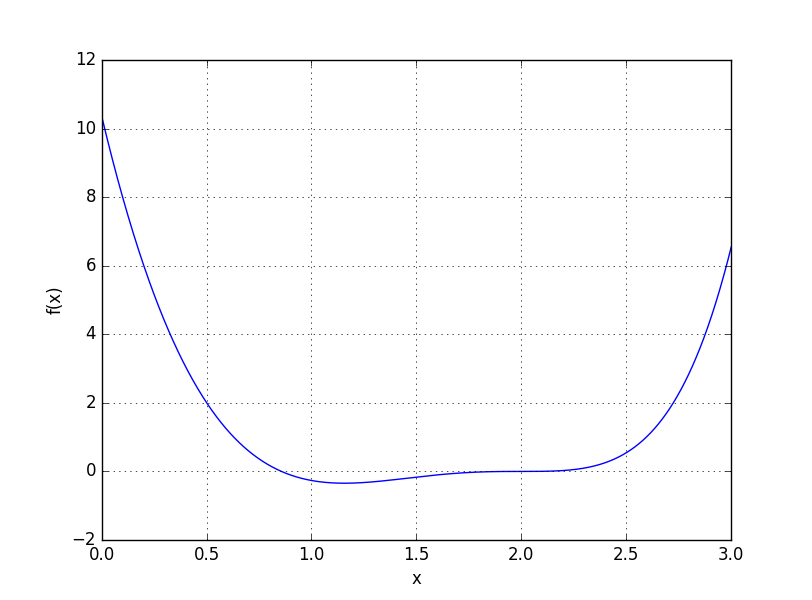
\includegraphics[scale = 0.8]{plot.png}
\end{center}

Στο πρώτο κομάτι της άσκησης η προσέγγιση της ρίζας γίνετε με την μέθοδο της διχοτόμησης:

\lstinputlisting[firstline=20, lastline=36, firstnumber=20]{ex1.py}

\begin{lstlisting}[language=bash, numbers=none, mathescape=true]
$\dollar$ python ex1.py
$\dollar$ f(0.952374) = 0.000000
\end{lstlisting}

Στην συνέχεια υπολογίζω τις ρίζες με την μέθοδο Newton-Raphson:

A change!
\end{document}

%%% Local Variables:
%%% coding: utf-8
%%% mode: latex
%%% TeX-engine: xetex
%%% End: